\newpage
\section{NOSQL (Not Only SQL)}


% Introduzione
\subsection{Introduzione}

Sono dei \hl{database distributi} con:

\begin{itemize}
    \item storage semistrutturato
    \item alta replicazione dei dati
    \item alte prestazioni
\end{itemize}

Non sarà richiesto uno schema ER, e ha come \hl{tipi}:

\begin{itemize}
    \item documentali
    \item chiave valore
    \item colonnari
    \item a grafo
    \item ibridi
    \item a oggetti
    \item xml
\end{itemize}


% CAP Theorem
\subsection{CAP Theorem}

Se ho modelli diversi di DB vorrei poter avere \hl{diversi livelli di consistenza dello stato del DB} e voler forzare la transazione. Allora dovremo avere:

\begin{itemize}
    \item \hl{consistenza}: in tutti i DB distribuiti \textbf{ciscuna istanza deve fornire gli stessi dati}
    \item \hl{disponibilita'}: \textbf{un fail del nodo master non deve intaccare gli altri}
    

    \begin{figure}[H]
    \centering
    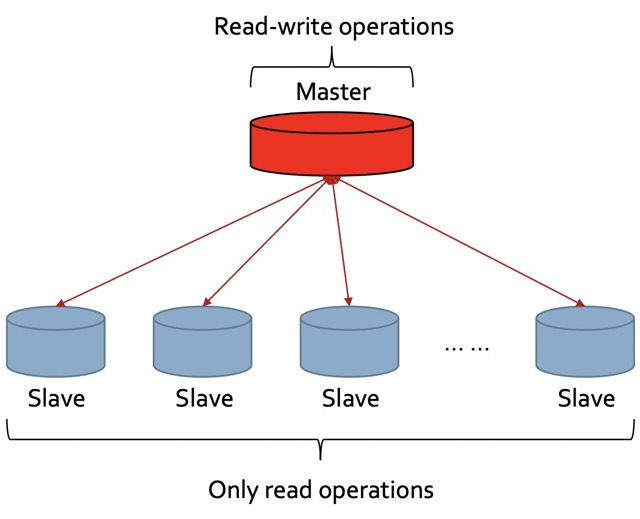
\includegraphics[scale=0.4]{masterslave.jpeg}
    \caption{Master and sleave} 
    \label{masterslave}
    \end{figure}


    \item \hl{partizione}: il sistema continua a \textbf{funzionare nonostante la perdita di messaggi, o problemi di connessione}
\end{itemize}

Se ho un sistema distribuito \hl{non possono garatire tutte e 3 le cose}, allora possono essere garantite \hl{solo 2 alla volta}:

\begin{figure}[H]
\centering
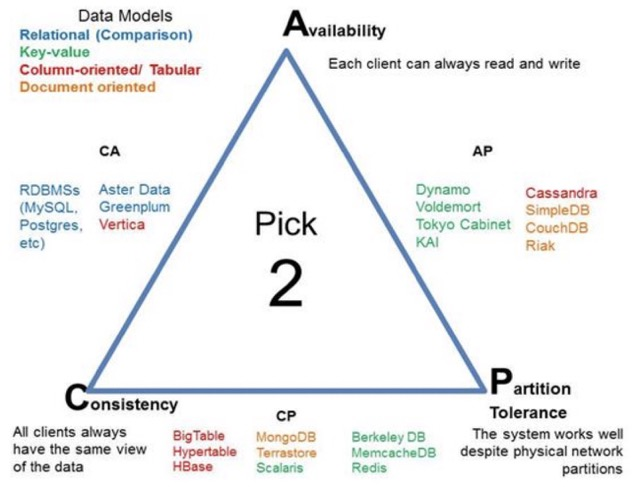
\includegraphics[scale=0.4]{cap.jpeg}
\caption{CAP theorem} 
\label{cap}
\end{figure}